%-----------------------------------------------------------------
%	PERFORMANCE
%	!TEX root = ./../main.tex
%-----------------------------------------------------------------
\section{Analysis of 2D Laplace program}\label{sec:results-laplace}

%-----------------------------------------------------------------
\subsection{CPU versions of the program}
To ease the work with the different versions of the code, we will use a systematic naming structure for the source codes, the binaries, and the logs:
\begin{itemize}
	\item \inline{lapCPU[#number]-description.c}
	\item \inline{lapCPU[#number]}
	\item \inline{lapCPU[#number]-perf.log}
\end{itemize}

This systematic naming convention will allow us to analyse the results easily using bash, AWK (using \inline{extract_perf.awk}), and R.

%---------------------------------
\subsubsection{Baseline \texttt{laplace2d.c} (\texttt{lapCPU1})}
First of all, we use the baseline \inline{laplace2d.c} program as provided by the professors:
\begin{lstlisting}[language=bash]
pgcc -lm -fast -Minfo=all lapCPU1-baseline.c -o lapCPU1
perf stat ./lapCPU1 250 2> lapCPU1-perf.log
\end{lstlisting}

The PGI compiler performs a series of optimisations on the code generated for CPU. The most relevant performance metrics are the elapsed execution time (\SI{135.33}{\s}), the total number of executed machine instructions (\num{40.26e9}), and the IPC rate (\num{0.09}).

%---------------------------------
\subsubsection{Baseline \texttt{lapFusion} (\texttt{lapCPU2} \& \texttt{lapCPU3})}
The second analysed version of the code is using the baseline \inline{lapFusion.c} program as provided by the professors:
\begin{lstlisting}[language=bash]
pgcc -lm -fast -openmp -Minfo=all lapCPU2-Fusion-baseline.c -o lapCPU2
perf stat ./lapCPU2 4096 250 2> lapCPU2-perf.log
\end{lstlisting}

The execution time is significantly reduced from \SI{135.33}{\s} to \SI{17.06}{\s}, but the total number of executed instructions is multiplied by 2.75 (\num{109.06e9}). This is something that we must check. A detailed look at the output from the PGI compiler reveals that the optimised code is not vectorized, even with the OpenMP \inline{#pragma} that confirms that the loop in line 23 is vectorisable.

In order to improve the task of the compiler, we include the \inline{inline} keyword before the declaration of functions \inline{stencil()} and \inline{max_error()} in the \inline{lapFusion.c} code, and it is compiled and executed again:
\begin{lstlisting}[language=bash]
pgcc -lm -fast -openmp -Minfo=all lapCPU3-Fusion-good.c -o lapCPU3
perf stat ./lapCPU3 4096 250 2> lapCPU3-perf.log
\end{lstlisting}

Again, the execution time is reduced from \SI{17.06}{\s} to \SI{9.43}{\s}, and the total number of executed instructions is almost halved (\num{56.66e9}), but still the optimised code is not vectorised. The compiler is not able to make a good analysis of the data dependencies when the matrices are represented as one-dimensional vectors and the elements are addressed using complex expressions.

Instead of trying to improve the output from the PGI compiler we opt by using the GCC compiler.

%---------------------------------
\subsubsection{Parallelised \texttt{lapFusion} using OpenMP (\texttt{lapCPU4})}
First of all, we need to load the GCC compiler into the system:
\begin{lstlisting}[language=bash]
module load gcc/7.2.0
\end{lstlisting}

Now, we create a parallelised version of the \inline{lapFusion} code using the following \inline{#pragma} directives:
\begin{lstlisting}[firstnumber=24]
  #pragma omp parallel for num_threads(3)
  for ( j=1; j < n-1; j++ )
	#pragma omp simd reduction(max:error)
	for ( i=1; i < n-1; i++ )
\end{lstlisting}

Then we compile using the GCC compiler and execute as usual:
\begin{lstlisting}[language=bash]
gcc -Ofast -lm -fopenmp lapCPU4-Fusion-parallel.c -o lapCPU4
perf stat ./lapCPU4 4096 250 2> lapCPU4-perf.log
\end{lstlisting}

Notice that using the \inline{inline} keyword has a very small influence on the execution time when vectorising the code using OpenMP.

The execution with three threads for 250 convergence loop iterations is about $2.2$ times faster than using a single thread and the operations have indeed been divided by 3 (\num{19.24e9}).

The fact that the performance does not scale linearly with the number of threads indicates that there is a performance problem. Since the total number of instructions executed is almost the same, the problem is an unexpected reduction of the IPC rate: some instructions are executed slower when using three processing cores than when using only one core. The explanation is that the DRAM memory bandwidth is almost exhausted with a single thread, and therefore the performance is bounded by the peak bandwidth of the DRAM memory.

%---------------------------------
\subsubsection{Comparison of the CPU versions}
In figure \ref{fig:times-cpu} below we can see a visual comparison of the execution times of the CPU versions of the Laplace program. The execution time is computed for \num{10000} iterations of the convergence loop, which is extrapolated by multiplying by 40 the time for executing 250 iterations of the convergence loop.
\begin{figure}[H]
	\centering
	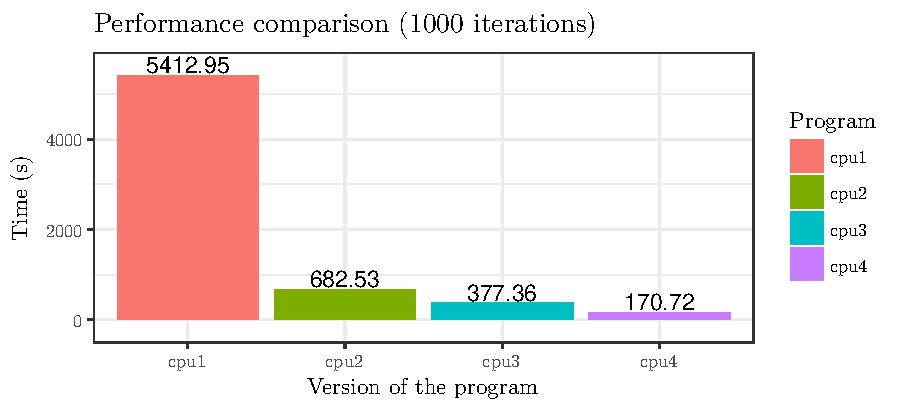
\includegraphics[width=0.9\textwidth]{images/times-cpu}
	\caption{Execution times of the CPU versions of the program}
	\label{fig:times-cpu}
\end{figure}

In the figure we can clearly see how each of the improvements has resulted in a reduction of the compilation time, specially the change from the sequential \inline{laplace2d.c} version to the \inline{lapFusion.c} version.

%-----------------------------------------------------------------
\subsection{GPU versions of the program}
To ease the work with the different versions of the code, we will use a systematic naming structure for the source codes, the binaries, and the compiler and profiler logs:
\begin{itemize}
	\item \inline{lapGPU[#number]-description.c}
	\item \inline{lapGPU[#number]}
	\item \inline{lapGPU[#number]-comp.log}
	\item \inline{lapGPU[#number]-nvp.log}
	\item \inline{lapGPU[#number]-metrics.log}
\end{itemize}

This systematic naming convention will allow us to analyse the results easily using bash, AWK (using \inline{extract_nvp.awk}), and R.

%---------------------------------
\subsubsection{Baseline (\texttt{lapGPU1})}
For this part, we will make our modifications using \inline{#pragma} directives on the \inline{laplace2d.c} code.

\begin{lstlisting}[firstnumber=77]
while ( error > tol && iter < iter_max )
{
	#pragma acc kernels
	for( i=1; i < m-1; i++ )
		for( j=1; j < n-1; j++)
			Anew[j][i] = ( A[j][i+1]+A[j][i-1]+A[j-1][i]+A[j+1][i]) / 4;

	error = 0.f;
	#pragma acc kernels
	for( i=1; i < m-1; i++ )
		for( j=1; j < n-1; j++)
			error = fmaxf( error, sqrtf( fabsf( Anew[j][i]-A[j][i] ) ) );

	#pragma acc kernels
	for( i=1; i < m-1; i++ )
		for( j=1; j < n-1; j++)
			A[j][i] = Anew[j][i];

	iter++;
	if(iter % (iter_max/10) == 0) printf("%5d, %0.6f\n", iter, error);
}
\end{lstlisting}

Since we will use the GPU for the calculations, we must use the PGI compiler:
\begin{lstlisting}[language=bash]
pgcc -fast -acc -ta=tesla:cc30 -Minfo=accel lapGPU1-baseline.c -o lapGPU1 &> lapGPU1-comp.log
\end{lstlisting}

Then we can use \inline{nvprof} to extract performance stats and some useful metrics:
\begin{lstlisting}[language=bash]
nvprof ./lapGPU1 10000 2> lapGPU1-nvp.log
nvprof --kernels "main_82_gpu" --metrics sm_activity,inst_executed,l2_utilization, dram_utilization,dram_read_throughput,dram_write_throughput,ipc ./lapGPU1 100 2> lapGPU1-metrics.log
\end{lstlisting}

The first thing to notice is that if we only use \inline{#pragma acc kernels} directives before each of the loops, most of the computation time is wasted on copying memory from the CPU to the GPU (and the other way around) for each iteration, as seen in figure~\ref{fig:timeline-gpu1b} below.
\begin{figure}[H]
	\centering
	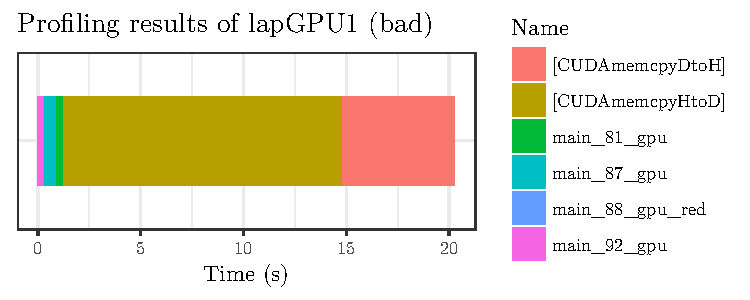
\includegraphics[width=0.7\textwidth]{images/timeline-gpu1b}
	\caption{Timeline of the execution time of the GPU1 version (bad), for 250 iterations}
	\label{fig:timeline-gpu1b}
\end{figure}

To fix this, we also need to include the following \inline{#pragma} directive before the main \inline{while} loop to tell the program that the GPU already has all the variables; this way the memory is only copied once from the CPU to the GPU at the beginning, and from the GPU to the CPU when the program finishes:
\begin{lstlisting}[firstnumber=77]
#pragma acc data copyin(A,Anew)
while ( error > tol && iter < iter_max )
\end{lstlisting}

In this way, we reduce the copying time to a bare minimum, as seen in figure~\ref{fig:timeline-gpu1} below. Even though we do 40 times the amount of iterations, the time is only doubled. This is a clear indication that we are using the GPU almost purely for calculations.
\begin{figure}[H]
	\centering
	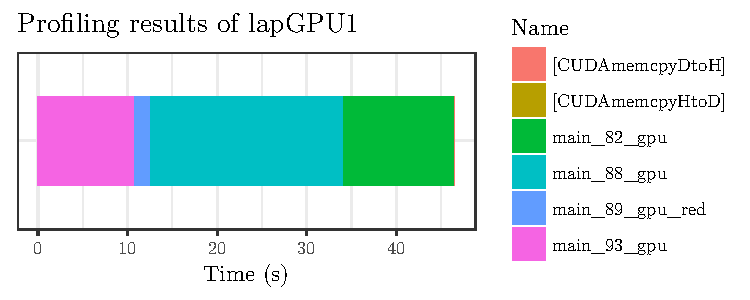
\includegraphics[width=0.7\textwidth]{images/timeline-gpu1}
	\caption{Timeline of the execution time of the GPU1 version, for \num{10000} iterations}
	\label{fig:timeline-gpu1}
\end{figure}

%---------------------------------
\subsubsection{Optimisation: loop fusion (\texttt{lapGPU2})}

For this version of the program, we fuse the loop for the calculation of the next step and the error into one single loop:
\begin{lstlisting}[firstnumber=81]
#pragma acc kernels
		for( i=1; i < m-1; i++ )
			for( j=1; j < n-1; j++){
				Anew[j][i] = ( A[j][i+1]+A[j][i-1]+A[j-1][i]+A[j+1][i]) / 4;
				error = fmaxf( error, sqrtf( fabsf( Anew[j][i]-A[j][i] ) ) );}
\end{lstlisting}

Then we compile with the PGI compiler as usual, and extract performance and metrics information:
\begin{lstlisting}[language=bash]
pgcc -fast -acc -ta=tesla:cc30 -Minfo=accel lapGPU2-loopfusion.c -o lapGPU2 &> lapGPU2-comp.log
nvprof ./lapGPU2 10000 2> lapGPU2-nvp.log
nvprof --kernels "main_82_gpu" --metrics sm_activity,inst_executed,l2_utilization, dram_utilization,dram_read_throughput,dram_write_throughput,ipc ./lapGPU2 100 2> lapGPU2-metrics.log
\end{lstlisting}

In figure~\ref{fig:timeline-gpu2} below we can clearly see how the two loops have been fused into one single operation, and how this fused operation is faster than the two operations by themselves in figure~\ref{fig:timeline-gpu1}. Notice that the reduction operation and the one done in \inline{main_93_gpu} have essentially the same duration in both implementations.
\begin{figure}[H]
	\centering
	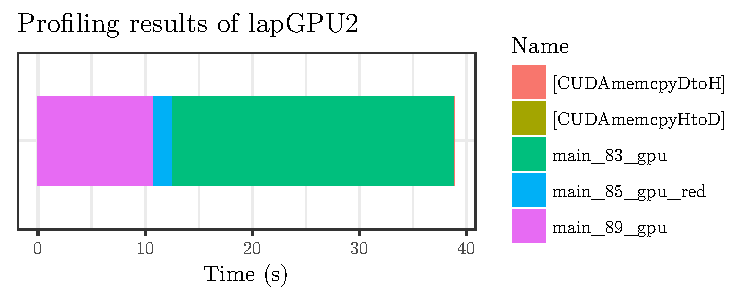
\includegraphics[width=0.7\textwidth]{images/timeline-gpu2}
	\caption{Timeline of the execution time of the GPU2 version, for \num{10000} iterations}
	\label{fig:timeline-gpu2}
\end{figure}

%---------------------------------
\subsubsection{Optimisation: loop interchange (\texttt{lapGPU3})}
For this version, we just exchange the order of the nested loops in lines \numrange{82}{83} and \numrange{88}{89}:
\begin{minipage}{.45\textwidth}
\begin{lstlisting}[firstnumber=81]
for( i=1; i < m-1; i++ )
	for( j=1; j < n-1; j++){
\end{lstlisting}
\end{minipage}%
\begin{minipage}{0.1\textwidth}
$\,\,\quad\mapsto$
\end{minipage}%
\begin{minipage}{0.45\textwidth}
\begin{lstlisting}[firstnumber=81]
for( j=1; j < n-1; j++ )
	for( i=1; i < m-1; i++){
\end{lstlisting}
\end{minipage}

Then we compile with the PGI compiler as usual, and extract performance and metrics information:
\begin{lstlisting}[language=bash]
pgcc -fast -acc -ta=tesla:cc30 -Minfo=accel lapGPU3-loopinter.c -o lapGPU3 &> lapGPU3-comp.log
nvprof ./lapGPU3 10000 2> lapGPU3-nvp.log
nvprof --kernels "main_83_gpu" --metrics sm_activity,inst_executed,l2_utilization, dram_utilization,dram_read_throughput,dram_write_throughput,ipc ./lapGPU3 100 2> lapGPU3-metrics.log
\end{lstlisting}

Having a look at figure~\ref{fig:timeline-gpu3} below and comparing it to figure~\ref{fig:timeline-gpu2}, we see no major improvements; one could even say that the performance is a bit worse.
\begin{figure}[H]
	\centering
	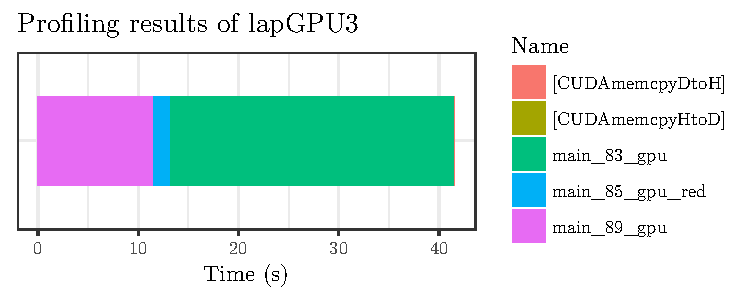
\includegraphics[width=0.7\textwidth]{images/timeline-gpu3}
	\caption{Timeline of the execution time of the GPU3 version, for \num{10000} iterations}
	\label{fig:timeline-gpu3}
\end{figure}

The reason for not being any major improvement is that the PGI compiler already knows the “good” order of the loops when it compiles the program.

%---------------------------------
\subsubsection{Optimisation: \texttt{sqrt} out of the loop (\texttt{lapGPU4})}
For this version, we move the $\sqrt{\texttt{error}}$ outside of the loop, since we do not need to know the square root of the intermediate errors, just the final error:
\begin{lstlisting}[firstnumber=82]
for( i=1; i < m-1; i++ )
	for( j=1; j < n-1; j++){
		Anew[j][i] = ( A[j][i+1]+A[j][i-1]+A[j-1][i]+A[j+1][i]) / 4;
		error = fmaxf( error, fabsf( Anew[j][i]-A[j][i] ) ) ;}
error = sqrtf(error);
\end{lstlisting}

Then we compile with the PGI compiler as usual, and extract performance and metrics information:
\begin{lstlisting}[language=bash]
pgcc -fast -acc -ta=tesla:cc30 -Minfo=accel lapGPU4-sqrt.c -o lapGPU4 &> lapGPU4-comp.log
nvprof ./lapGPU4 10000 2> lapGPU4-nvp.log
nvprof --kernels "main_83_gpu" --metrics sm_activity,inst_executed,l2_utilization, dram_utilization,dram_read_throughput,dram_write_throughput,ipc ./lapGPU4 100 2> lapGPU4-metrics.log
\end{lstlisting}

This improvement just has a small impact on the execution time, as seen in figure~\ref{fig:timeline-gpu4}.
\begin{figure}[H]
	\centering
	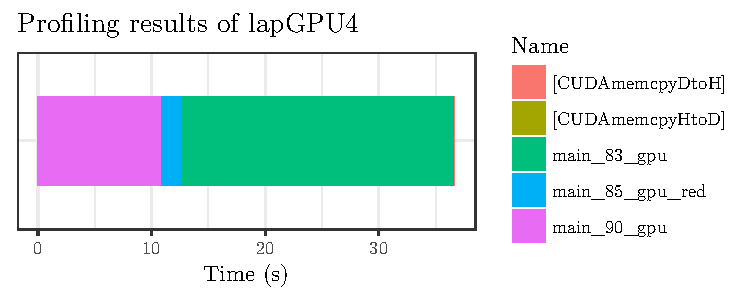
\includegraphics[width=0.7\textwidth]{images/timeline-gpu4}
	\caption{Timeline of the execution time of the GPU4 version, for \num{10000} iterations}
	\label{fig:timeline-gpu4}
\end{figure}

As a summary of these last versions, we can say that versions 2 and 3 are essentially the same, because the compiler already manages to optimise the order of the loops. and Version 4 does not add much to the performance, because of the limitation of the DRAM bandwidth.

%---------------------------------
\subsubsection{Optimisation: double buffer (\texttt{lapGPU5})}
For this version, is to use a double buffer. This allows us to avoid copying from \inline{Anew} to \inline{A} by reversing roles of \inline{A} and \inline{Anew} on every iteration:
\begin{lstlisting}[firstnumber=81]
if(iter % 2 == 0){
	#pragma acc kernels
	for( j=1; j < n-1; j++){
		for( i=1; i < m-1; i++ ){
			Anew[j][i] = ( A[j][i+1]+A[j][i-1]+A[j-1][i]+A[j+1][i])*0.25f;
			error = fmaxf( error, fabsf( Anew[j][i]-A[j][i] ) );}}
} else{
	#pragma acc kernels
	for( j=1; j < n-1; j++){
		for( i=1; i < m-1; i++ ){
			A[j][i] = ( Anew[j][i+1]+Anew[j][i-1]+Anew[j-1][i]+Anew[j+1][i])*0.25f;
			error = fmaxf( error, fabsf( A[j][i]-Anew[j][i] ) );}}
}
\end{lstlisting}

Then we compile with the PGI compiler as usual, and extract performance and metrics information:
\begin{lstlisting}[language=bash]
pgcc -fast -acc -ta=tesla:cc30 -Minfo=accel lapGPU5-double.c -o lapGPU5 &> lapGPU5-comp.log
nvprof ./lapGPU5 10000 2> lapGPU5-nvp.log
nvprof --kernels "main_84_gpu" --metrics sm_activity,inst_executed,l2_utilization, dram_utilization,dram_read_throughput,dram_write_throughput,ipc ./lapGPU5 100 2> lapGPU5-metrics.log
\end{lstlisting}

This is the next major improvement next to the loop fusion. In figure~\ref{fig:timeline-gpu5} we can clearly see how the execution is divided into two processes of computation and reduction. This is a clear indication that the double buffer works as intended.
\begin{figure}[H]
	\centering
	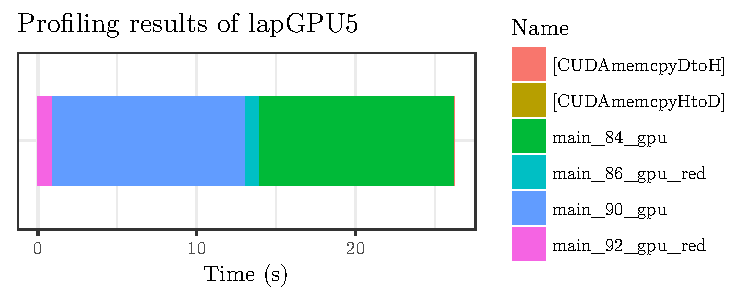
\includegraphics[width=0.7\textwidth]{images/timeline-gpu5}
	\caption{Timeline of the execution time of the GPU5 version, for \num{10000} iterations}
	\label{fig:timeline-gpu5}
\end{figure}

%---------------------------------
\subsubsection{Optimisation: parallel loop (vector 128) (\texttt{lapGPU6})}
Looking at \inline{lapGPU5-comp.log} we see we can still make a small optimisation to reduce the execution time: adding \inline{vector_length(128)} to the \inline{#pragma acc kernels} directives in lines 82 and 88 to force the size of the parallel loop:
\begin{lstlisting}[firstnumber=82]
#pragma acc kernels vector_length(128)
\end{lstlisting}

With this we make sure to divide the GPU into threads of the appropriate size to fully take advantage of our hardware.

Then we compile with the PGI compiler as usual, and extract performance and metrics information:
\begin{lstlisting}[language=bash]
pgcc -fast -acc -ta=tesla:cc30 -Minfo=accel lapGPU6-vec128.c -o lapGPU6 &> lapGPU6-comp.log
nvprof ./lapGPU6 10000 &> lapGPU6-nvp.log
nvprof --kernels "main_84_gpu" --metrics sm_activity,inst_executed,l2_utilization, dram_utilization,dram_read_throughput,dram_write_throughput,ipc ./lapGPU6 100 2> lapGPU6-metrics.log
\end{lstlisting}

In figure~\ref{fig:timeline-gpu6} we can see how the functioning to figure~\ref{fig:timeline-gpu5} is essentially the same. We just get a small time improvement.
\begin{figure}[H]
	\centering
	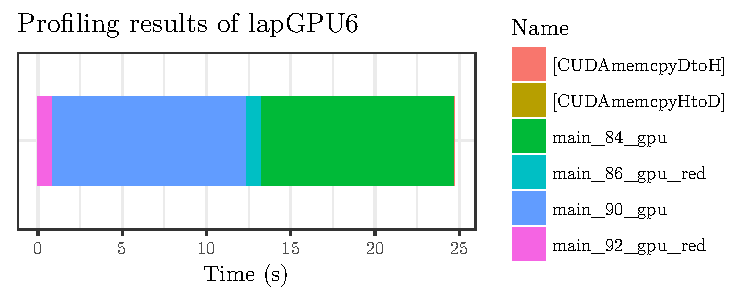
\includegraphics[width=0.7\textwidth]{images/timeline-gpu6}
	\caption{Timeline of the execution time of the GPU6 version, for \num{10000} iterations}
	\label{fig:timeline-gpu6}
\end{figure}

%---------------------------------
\subsubsection{Comparison of the GPU versions}
\begin{figure}[H]
	\centering
	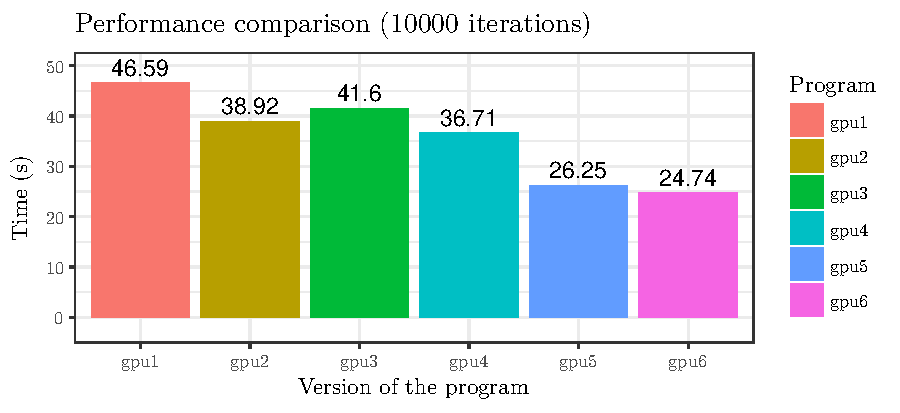
\includegraphics[width=0.9\textwidth]{images/times-gpu}
	\caption{Execution times of the GPU versions of the program}
	\label{fig:times-gpu}
\end{figure}

If we take a look at figure~\ref{fig:times-gpu}, we can compare the different implementations of GPU-oriented parallelisation and address its different results. It is relevant to note that not all implementations have been equally useful; as a matter of fact, some of them have been even counter-productive. Therefore, we  must consider the characteristics of the best implementations individually and highlight its importance.

The great improvements in the performance when using these different implementations are observed  in \inline{lapGPU2} and \inline{lapGPU5}. The former fuses different loops into a single loops, considerably reducing the operations needed to perform the same results; whilst the latter uses a double buffer in order to avoid carrying big matrices more times that needed, releasing a great deal of memory and hence easing the overall computation.

%---------------------------------
\subsubsection{Summary of the metrics}

In table~\ref{tab:metrics} below we can see a few conclusions can be extracted:
\begin{itemize}
	\item The biggest change is when implementing the loop fusion (\inline{GPU2}). The executed instructions are almost doubled, whilst the DRAM read/write throughput is halved. The IPC rate is a bit worse, but that does not have an important impact on the performance.
	\item For some reason, the loop inversion (\inline{GPU3}) has a pretty important, and bad, result on the performance as well as the metrics. The executed instructions were increased when compared to \inline{GPU2}, being this probably the reason of the increase in the execution time.
	\item Moving the square root out of the loop (\inline{GPU5}) improves a bit the DRAM read/write throughput and reduces the amount of executed instructions, as expected.
	\item Using the double buffer (\inline{GPU5}), even though makes a great performance improvement, does not make a big change on the metrics.
	\item Forcing the size of the parallel loop (\texttt{GPU6}) to 128 not only reduces the execution time, but the total executed instructions whilst improving the IPC rate.
\end{itemize}

\begin{table}[H]
	\centering
	\resizebox{\textwidth}{!}{
	\begin{tabular}{l c c c c c c}
	\toprule
	\toprule
	Version of the Program     & \texttt{GPU1}  & \texttt{GPU2}  & \texttt{GPU3}  & \texttt{GPU4}  & \texttt{GPU5}  & \texttt{GPU6}  \\
	\midrule
	Instructions Executed      & \num{24105472} & \num{46363722} & \num{50047882} & \num{43117312} & \num{43117312} & \num{41005504} \\
	L2 Cache Utilization       & Mid (6)        & Mid (4)        & Mid (4)        & Mid (4)        & Mid (4)        & Mid (4)        \\
	DRAM Utilization           & Mid (6)        & Low (3)        & Low (3)        & Low (3)        & Low (3)        & Mid (4)        \\
	DRAM Read (\si{GB\per\s})  & \num{50.161}   & \num{23.281}   & \num{23.149}   & \num{24.653}   & \num{24.658}   & \num{26.781}   \\
	DRAM Write (\si{GB\per\s}) & \num{51.078}   & \num{24.181}   & \num{23.979}   & \num{26.454}   & \num{26.455}   & \num{27.929}   \\
	Executed IPC               & \num{2.253070} & \num{2.001180} & \num{1.983949} & \num{1.972142} & \num{1.972746} & \num{2.037747} \\
	Multiprocessor Activity    & 99.72\%        & 99.86\%        & 99.87\%        & 99.86\%        & 99.86\%        & 99.85\%        \\
	\bottomrule
	\bottomrule
	\end{tabular}}
	\caption{Summary of the average metrics obtained with \inline{nvprof} for the different implementations of the program for GPU}
	\label{tab:metrics}
\end{table}

%-----------------------------------------------------------------
\subsection{Comparison of CPU vs GPU versions}
Until now we have discussed the different implementations used within a CPU-oriented parallelisation and their compared performances; nextly, we have stutdied the different implementations employed within a GPU-oriented parallelisation. Now it would be interesting to contrast the performances acquired between all different CPU and GPU oriented parallelisation implementations.
\begin{figure}[H]
	\centering
	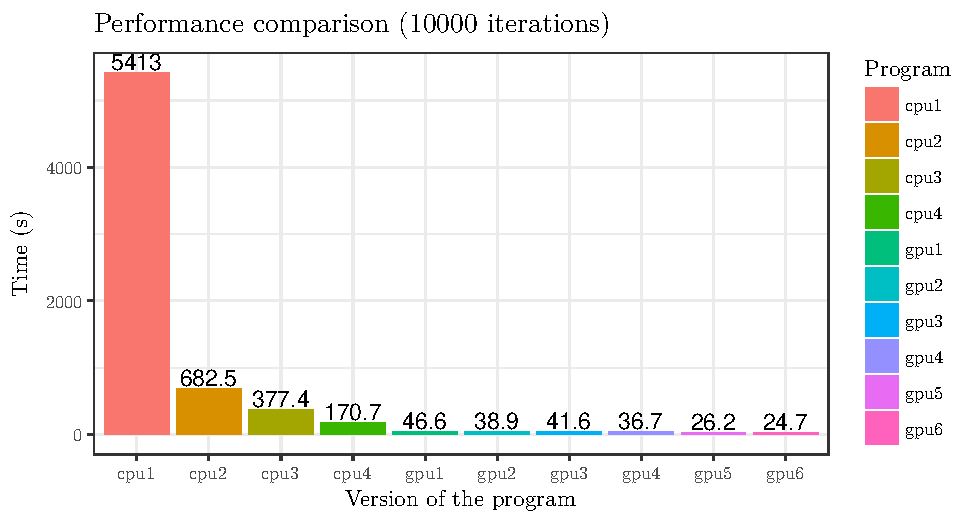
\includegraphics[width=0.95\textwidth]{images/times-all}
	\caption{Execution times of the CPU and GPU versions of the program}
	\label{fig:times-all}
\end{figure}

On figure~\ref{fig:times-all} above it is shown the execution times of all the different versions of the program. If we look closely at the figure, it is quite clear how dwarfed are the differences between the particular versions, when taking into account whether the version is CPU-oriented or GPU-oriented. The general conclusion extracted from this graph is that no matter how well implemented is a CPU parallelisation, the worst implementation using GPU is far better and it consumes considerably less computation time.

Despite that, some great improvements can be -- and should be -- acknowledged when well-implemented CPU parallelisation is used. This highlights the importance of a thorough parallelisation of the code, specially when no GPU is available.



